\begin{figure}
\vspace{-4pt}
    \begingroup
    \setlength{\tabcolsep}{1pt}
    \centering
    \begin{tabular}{cccc}
        & \smaller{CIFAR-100 (1 Image / Class)} & & \smaller{CIFAR-100 (1 Image / Class)}\\
        \rotatebox[origin=c]{90}{\smaller{Validation Acc. \%}} &  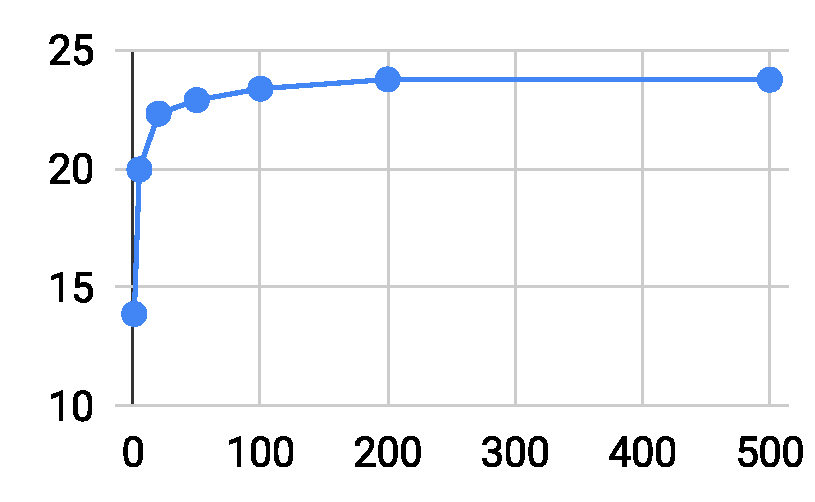
\includegraphics[align=c,width=0.43\linewidth]{figures/experts.pdf}& \hfill\;\;\;\;\rotatebox[origin=c]{90}{\smaller{Validation Acc. \%}} &  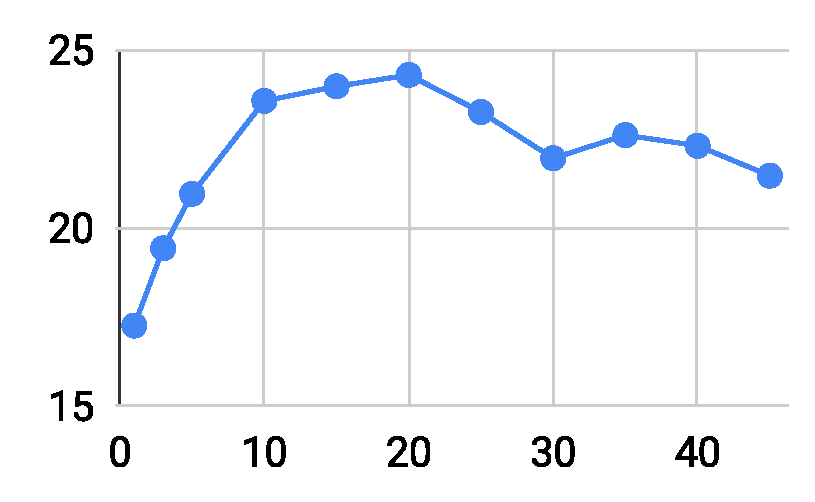
\includegraphics[align=c,width=0.43\linewidth]{figures/start-epoch.pdf}\\
         & \smaller{\;\;\;\;\;\# Expert Trajectories} & & \smaller{\;\;$T^+$: Max Start Epoch}
    \end{tabular}
    \endgroup
        \vspace{-7pt}
    \caption{\textbf{Left:} We see logarithmic performance improvement with respect to the number of expert trajectories used, quickly saturating near 200. \textbf{Right:} The upper bound on the expert epoch at which the synthetic data starts working cannot be too high or low to ensure quality learning signal.}
    \lblfig{experts}
    \vspace{-10pt}
\end{figure}
